% Options for packages loaded elsewhere
\PassOptionsToPackage{unicode}{hyperref}
\PassOptionsToPackage{hyphens}{url}
%
\documentclass[
]{article}
\usepackage{lmodern}
\usepackage{amssymb,amsmath}
\usepackage{ifxetex,ifluatex}
\ifnum 0\ifxetex 1\fi\ifluatex 1\fi=0 % if pdftex
  \usepackage[T1]{fontenc}
  \usepackage[utf8]{inputenc}
  \usepackage{textcomp} % provide euro and other symbols
\else % if luatex or xetex
  \usepackage{unicode-math}
  \defaultfontfeatures{Scale=MatchLowercase}
  \defaultfontfeatures[\rmfamily]{Ligatures=TeX,Scale=1}
\fi
% Use upquote if available, for straight quotes in verbatim environments
\IfFileExists{upquote.sty}{\usepackage{upquote}}{}
\IfFileExists{microtype.sty}{% use microtype if available
  \usepackage[]{microtype}
  \UseMicrotypeSet[protrusion]{basicmath} % disable protrusion for tt fonts
}{}
\makeatletter
\@ifundefined{KOMAClassName}{% if non-KOMA class
  \IfFileExists{parskip.sty}{%
    \usepackage{parskip}
  }{% else
    \setlength{\parindent}{0pt}
    \setlength{\parskip}{6pt plus 2pt minus 1pt}}
}{% if KOMA class
  \KOMAoptions{parskip=half}}
\makeatother
\usepackage{xcolor}
\IfFileExists{xurl.sty}{\usepackage{xurl}}{} % add URL line breaks if available
\IfFileExists{bookmark.sty}{\usepackage{bookmark}}{\usepackage{hyperref}}
\hypersetup{
  pdftitle={Single\_effect},
  pdfauthor={Jungang Zou},
  hidelinks,
  pdfcreator={LaTeX via pandoc}}
\urlstyle{same} % disable monospaced font for URLs
\usepackage[margin=1in]{geometry}
\usepackage{color}
\usepackage{fancyvrb}
\newcommand{\VerbBar}{|}
\newcommand{\VERB}{\Verb[commandchars=\\\{\}]}
\DefineVerbatimEnvironment{Highlighting}{Verbatim}{commandchars=\\\{\}}
% Add ',fontsize=\small' for more characters per line
\usepackage{framed}
\definecolor{shadecolor}{RGB}{248,248,248}
\newenvironment{Shaded}{\begin{snugshade}}{\end{snugshade}}
\newcommand{\AlertTok}[1]{\textcolor[rgb]{0.94,0.16,0.16}{#1}}
\newcommand{\AnnotationTok}[1]{\textcolor[rgb]{0.56,0.35,0.01}{\textbf{\textit{#1}}}}
\newcommand{\AttributeTok}[1]{\textcolor[rgb]{0.77,0.63,0.00}{#1}}
\newcommand{\BaseNTok}[1]{\textcolor[rgb]{0.00,0.00,0.81}{#1}}
\newcommand{\BuiltInTok}[1]{#1}
\newcommand{\CharTok}[1]{\textcolor[rgb]{0.31,0.60,0.02}{#1}}
\newcommand{\CommentTok}[1]{\textcolor[rgb]{0.56,0.35,0.01}{\textit{#1}}}
\newcommand{\CommentVarTok}[1]{\textcolor[rgb]{0.56,0.35,0.01}{\textbf{\textit{#1}}}}
\newcommand{\ConstantTok}[1]{\textcolor[rgb]{0.00,0.00,0.00}{#1}}
\newcommand{\ControlFlowTok}[1]{\textcolor[rgb]{0.13,0.29,0.53}{\textbf{#1}}}
\newcommand{\DataTypeTok}[1]{\textcolor[rgb]{0.13,0.29,0.53}{#1}}
\newcommand{\DecValTok}[1]{\textcolor[rgb]{0.00,0.00,0.81}{#1}}
\newcommand{\DocumentationTok}[1]{\textcolor[rgb]{0.56,0.35,0.01}{\textbf{\textit{#1}}}}
\newcommand{\ErrorTok}[1]{\textcolor[rgb]{0.64,0.00,0.00}{\textbf{#1}}}
\newcommand{\ExtensionTok}[1]{#1}
\newcommand{\FloatTok}[1]{\textcolor[rgb]{0.00,0.00,0.81}{#1}}
\newcommand{\FunctionTok}[1]{\textcolor[rgb]{0.00,0.00,0.00}{#1}}
\newcommand{\ImportTok}[1]{#1}
\newcommand{\InformationTok}[1]{\textcolor[rgb]{0.56,0.35,0.01}{\textbf{\textit{#1}}}}
\newcommand{\KeywordTok}[1]{\textcolor[rgb]{0.13,0.29,0.53}{\textbf{#1}}}
\newcommand{\NormalTok}[1]{#1}
\newcommand{\OperatorTok}[1]{\textcolor[rgb]{0.81,0.36,0.00}{\textbf{#1}}}
\newcommand{\OtherTok}[1]{\textcolor[rgb]{0.56,0.35,0.01}{#1}}
\newcommand{\PreprocessorTok}[1]{\textcolor[rgb]{0.56,0.35,0.01}{\textit{#1}}}
\newcommand{\RegionMarkerTok}[1]{#1}
\newcommand{\SpecialCharTok}[1]{\textcolor[rgb]{0.00,0.00,0.00}{#1}}
\newcommand{\SpecialStringTok}[1]{\textcolor[rgb]{0.31,0.60,0.02}{#1}}
\newcommand{\StringTok}[1]{\textcolor[rgb]{0.31,0.60,0.02}{#1}}
\newcommand{\VariableTok}[1]{\textcolor[rgb]{0.00,0.00,0.00}{#1}}
\newcommand{\VerbatimStringTok}[1]{\textcolor[rgb]{0.31,0.60,0.02}{#1}}
\newcommand{\WarningTok}[1]{\textcolor[rgb]{0.56,0.35,0.01}{\textbf{\textit{#1}}}}
\usepackage{graphicx,grffile}
\makeatletter
\def\maxwidth{\ifdim\Gin@nat@width>\linewidth\linewidth\else\Gin@nat@width\fi}
\def\maxheight{\ifdim\Gin@nat@height>\textheight\textheight\else\Gin@nat@height\fi}
\makeatother
% Scale images if necessary, so that they will not overflow the page
% margins by default, and it is still possible to overwrite the defaults
% using explicit options in \includegraphics[width, height, ...]{}
\setkeys{Gin}{width=\maxwidth,height=\maxheight,keepaspectratio}
% Set default figure placement to htbp
\makeatletter
\def\fps@figure{htbp}
\makeatother
\setlength{\emergencystretch}{3em} % prevent overfull lines
\providecommand{\tightlist}{%
  \setlength{\itemsep}{0pt}\setlength{\parskip}{0pt}}
\setcounter{secnumdepth}{-\maxdimen} % remove section numbering

\title{Single\_effect}
\author{Jungang Zou}
\date{4/28/2021}

\begin{document}
\maketitle

\begin{Shaded}
\begin{Highlighting}[]
\CommentTok{# import packages and define some useful mathematical functions}
\NormalTok{knitr}\OperatorTok{::}\NormalTok{opts_chunk}\OperatorTok{$}\KeywordTok{set}\NormalTok{(}\DataTypeTok{echo =} \OtherTok{TRUE}\NormalTok{)}
\KeywordTok{library}\NormalTok{(parallel)}
\KeywordTok{library}\NormalTok{(doParallel)}
\end{Highlighting}
\end{Shaded}

\begin{verbatim}
## Loading required package: foreach
\end{verbatim}

\begin{verbatim}
## Loading required package: iterators
\end{verbatim}

\begin{Shaded}
\begin{Highlighting}[]
\KeywordTok{library}\NormalTok{(foreach)}
\KeywordTok{library}\NormalTok{(}\StringTok{"MCMCpack"}\NormalTok{)}
\end{Highlighting}
\end{Shaded}

\begin{verbatim}
## Loading required package: coda
\end{verbatim}

\begin{verbatim}
## Loading required package: MASS
\end{verbatim}

\begin{verbatim}
## ##
## ## Markov Chain Monte Carlo Package (MCMCpack)
\end{verbatim}

\begin{verbatim}
## ## Copyright (C) 2003-2021 Andrew D. Martin, Kevin M. Quinn, and Jong Hee Park
\end{verbatim}

\begin{verbatim}
## ##
## ## Support provided by the U.S. National Science Foundation
\end{verbatim}

\begin{verbatim}
## ## (Grants SES-0350646 and SES-0350613)
## ##
\end{verbatim}

\begin{Shaded}
\begin{Highlighting}[]
\NormalTok{sigmoid =}\StringTok{ }\ControlFlowTok{function}\NormalTok{(x) }\KeywordTok{return}\NormalTok{(}\DecValTok{1} \OperatorTok{/}\StringTok{ }\NormalTok{(}\DecValTok{1} \OperatorTok{+}\StringTok{ }\KeywordTok{exp}\NormalTok{(}\OperatorTok{-}\NormalTok{x)))}

\NormalTok{softmax =}\StringTok{ }\ControlFlowTok{function}\NormalTok{(x)\{}
\NormalTok{  e_x =}\StringTok{ }\KeywordTok{exp}\NormalTok{(x }\OperatorTok{-}\StringTok{ }\KeywordTok{max}\NormalTok{(x))}
  \KeywordTok{return}\NormalTok{(e_x }\OperatorTok{/}\StringTok{ }\KeywordTok{sum}\NormalTok{(e_x))}
\NormalTok{\}}
\end{Highlighting}
\end{Shaded}

\hypertarget{genetic-association-selection-based-on-bayesian-methods}{%
\subsection{Genetic Association Selection based on Bayesian
Methods}\label{genetic-association-selection-based-on-bayesian-methods}}

Nowadays, statistical genetics is becoming more and more popular. It
uses statistical tools to find the statistical association between
disease(or phenotype) with a set of candidate genes, which provides a
pre-selection tool to Biologists. However, in genetic data, usually a
large amount of genes(genotype data) are provided for each sample, but
only few samples(each stands for an individual) are able to be
exploited. This special biological context can lead to a lot of problems
in statistical models, such as intensive computation, high dimension
curse, non-invertible normal matrix in ordinary least square. On the
other hand, Bayesian statistical method gives another framework to cope
with genetic association problems, which mixes up the information based
on personal belief and data. These kind of models are applied in
statistical genetic problems more and more frequently.

To solve the problems caused by genetic data, a lot of different methods
are proposed. The main ideas of these models are based on the fact that
we only need to identify the most significant genes instead of the whole
genetic dataset. In fact, a series of statistical methods built by
frequentists can be exploited for the same application purpose, such as
shrinkage method(Lasso for example), step-wise regression. These methods
can identify the covariates of the most statistical significance. Also,
in Bayesian framework, variable selection technique or model averaging
technique can be used. Bayesian variable selection methods specify
special prior distributions for parameters in regression, where the
inference based on posterior distributions will show whether this
covariate will be included in models. Among a broad range of priors, a
very useful prior is
\href{https://en.wikipedia.org/wiki/Spike-and-slab_regression}{Spike-Slab
prior}. On the other hand, Bayesian Model Averaging considers
probabilities of covariates subsets separately, instead of the whole
dataset. In this method, datasets are separated into different subsets
by columns, then regression models will be fitted on each subset of
variables. Finally, posterior probability of each model will be
calculated with the evidence of data. Generally speaking, there are
totally \(2^p\) models, \(p\) denotes the number of genes. To reduce the
intensive computation, ``single effect'' model is often specified, which
separates the whole data into only \(p\) different subsets and each
subset contains only one variable(gene). For Bayesian Model Averaging,
we consider the effect of only one gene separately, while the co-effect
of all genes will be applied in Bayesian Variable Selection.

In this notebook, we code 2 algorithms to identify significant genes
associated with phenotypes in R code, based on Bayesian Variable
Selection technique and Bayesian Model Averaging technique respectively.

\hypertarget{single-effect-logistic-regression-based-on-bayesian-model-averaging}{%
\subsubsection{Single Effect Logistic Regression based on Bayesian Model
Averaging}\label{single-effect-logistic-regression-based-on-bayesian-model-averaging}}

In our context of single effect logistic regression model, only one gene
will be included in regression. Formally, we can write down the
likelihood of j-th model:

\$p(y \textbar{} x\^{}j, \beta\_0\^{}j, \beta\_1\^{}j, M\^{}j)=
\prod\_i\textsuperscript{n(sigmoid(x\_i}j * \beta\_1\^{}j +
\beta\_0\textsuperscript{j))}\{y\_i\}(1 - sigmoid(x\_i\^{}j *
\beta\_1\^{}j + \beta\_0\textsuperscript{j))}\{1-y\_i\} \$, where
\(x^j\) is the j-th variable, \(x_i^j\) is j-th variable of i-th sample,
\(M^j\) gives this j-th model.

The process of Single Effect Bayesian Model Averaging(BMA) can be
followed by 5 steps: 1. Specify a prior inclusion probability for each
single effect model \(\pi(M_j),j=1,2...p\) with \(\sum_1^p\pi(M_j) = 1\)
constraint. 2. Specify prior of parameters in each model
\(\pi(\beta_0^j, \beta_1^j | M_j)\), then sample \(\beta_0^j\) and
\(\beta_1^j\) from prior distribution. 3. Calculate likelihood under
model
\(p(y |x^j, M_j ) = \int \int p(y|x^j, \beta_0^j, \beta_1^j, M_j) \pi(\beta_0^j, \beta_1^j | M_j) d\beta_0^jd\beta_1^j\)
by Monte Carlo integrals. 4. Calculate posterior inclusion probability
for each model by Bayes Rule
\(\pi(M_j | y, x^j) = \frac{\pi(M_j) *p(y |x^j, M_j ) }{\sum_1^p\pi(M_j) *p(y |x^j, M_j )}\).
5. Use MCMC or Variation Inference methods to infer posterior
distributions for each pair (\(\beta_0^j\), \(\beta_1^j\)), if needed.

\hypertarget{simple-bma-without-inference}{%
\paragraph{Simple BMA without
Inference}\label{simple-bma-without-inference}}

In most of the scenario of genetic association study, the effect of
parameters for significant genes is not rather important. Instead,
posterior inclusion probability(PIP) is what we concern about. Due to
this convenient situation, the algorithm without inference is typically
rapid, with no loop in the procedure.

In our algorithm, we specify a uniform distribution on user-defined
interval \([lower, higher]\) for \(\beta_0^j\), and user-defined normal
distribution \(Normal(\mu_0, \sigma_0^2)\) for \(\beta_1^j\). The code
of simple non-inference BMA method is as follow:

\begin{Shaded}
\begin{Highlighting}[]
\CommentTok{# calculate log-likelihood for a pair of parameters.}
\NormalTok{log_logistic_likelihood =}\StringTok{ }\ControlFlowTok{function}\NormalTok{(x, y, beta_}\DecValTok{0}\NormalTok{, beta_}\DecValTok{1}\NormalTok{, }\DataTypeTok{tol =} \FloatTok{1e-100}\NormalTok{)\{}
\NormalTok{  lm =}\StringTok{ }\NormalTok{beta_}\DecValTok{0} \OperatorTok{+}\StringTok{ }\NormalTok{beta_}\DecValTok{1} \OperatorTok{*}\StringTok{ }\NormalTok{x}
  \KeywordTok{return}\NormalTok{(}\KeywordTok{sum}\NormalTok{(y }\OperatorTok{*}\StringTok{ }\KeywordTok{log}\NormalTok{(}\KeywordTok{sigmoid}\NormalTok{(lm) }\OperatorTok{+}\StringTok{ }\NormalTok{tol) }\OperatorTok{+}\StringTok{ }\NormalTok{(}\DecValTok{1} \OperatorTok{-}\StringTok{ }\NormalTok{y) }\OperatorTok{*}\StringTok{ }\KeywordTok{log}\NormalTok{(}\DecValTok{1} \OperatorTok{-}\StringTok{ }\KeywordTok{sigmoid}\NormalTok{(lm) }\OperatorTok{+}\StringTok{ }\NormalTok{tol)))}
\NormalTok{\}}

\CommentTok{# the main algorithm of Bayesian Model Averaging}
\CommentTok{# Input:}
\CommentTok{# X: a matrix of genotype data. The process of centralization or normalization should be calculated before this algorithm if needed.}
\CommentTok{# Y: a vector of phenotype data, only binary data(0 or 1) is allowed. }
\CommentTok{# prior_ip: prior inclusion probability for each model. The size of vector should be consistent with variables of X. If prior_ip is not normalized(sum to 1), a process of normalization will be done in algorithm.}
\CommentTok{# mu0: a scalar to specify the prior normal mean of beta_1}
\CommentTok{# sigma0: a scalar to specify the prior normal standard deviation of beta_1}
\CommentTok{# lower: a scalar to specify the prior lower bound of uniform distribution for beta_0}
\CommentTok{# higher: a scalar to specify the prior upper bound of uniform distribution for beta_0}
\CommentTok{# sample_size: a scalar to specify the number of samples for parameters to perform Monte Carlo Integral for p(data | M_j)}

\CommentTok{# output:}
\CommentTok{# A vector of posterior inclusion probability for each variable.}

\NormalTok{BMA_simple =}\StringTok{ }\ControlFlowTok{function}\NormalTok{(X, Y, prior_ip, mu0, sigma0, lower, higher, }\DataTypeTok{sample_size =} \DecValTok{10000}\NormalTok{)\{}
  \CommentTok{# preparation}
\NormalTok{  n =}\StringTok{ }\KeywordTok{nrow}\NormalTok{(X)}
\NormalTok{  p =}\StringTok{ }\KeywordTok{ncol}\NormalTok{(X)}
  \ControlFlowTok{if}\NormalTok{(}\KeywordTok{length}\NormalTok{(prior_ip) }\OperatorTok{!=}\StringTok{ }\NormalTok{p)\{}
    \KeywordTok{stop}\NormalTok{(}\StringTok{"number of dimensions of prior inclusion probability and X are not consistent"}\NormalTok{)}
\NormalTok{  \}}
  \ControlFlowTok{if}\NormalTok{(}\KeywordTok{sum}\NormalTok{(prior_ip) }\OperatorTok{!=}\StringTok{ }\DecValTok{1}\NormalTok{)}
\NormalTok{    prior_ip =}\StringTok{ }\NormalTok{prior_ip }\OperatorTok{/}\StringTok{ }\KeywordTok{sum}\NormalTok{(prior_ip)}
  
  \CommentTok{# sample parameters}
\NormalTok{  beta_}\DecValTok{0}\NormalTok{ =}\StringTok{ }\KeywordTok{sapply}\NormalTok{(}\DecValTok{1}\OperatorTok{:}\NormalTok{p, }\ControlFlowTok{function}\NormalTok{(x)\{}\KeywordTok{runif}\NormalTok{(sample_size, lower, higher)\})}
\NormalTok{  beta_}\DecValTok{1}\NormalTok{ =}\StringTok{ }\KeywordTok{sapply}\NormalTok{(}\DecValTok{1}\OperatorTok{:}\NormalTok{p, }\ControlFlowTok{function}\NormalTok{(x)\{}\KeywordTok{rnorm}\NormalTok{(sample_size, mu0, sigma0)\})}
  
  \CommentTok{# calculate log-likelihood condition on only model}
\NormalTok{  logp_likelihood =}\StringTok{ }\KeywordTok{sapply}\NormalTok{(}\DecValTok{1}\OperatorTok{:}\NormalTok{p, }\ControlFlowTok{function}\NormalTok{(j)\{}
    \ControlFlowTok{if}\NormalTok{ (p }\OperatorTok{==}\StringTok{ }\DecValTok{1}\NormalTok{)\{}
\NormalTok{      beta_}\DecValTok{0}\NormalTok{_j =}\StringTok{ }\NormalTok{beta_}\DecValTok{0}
\NormalTok{      beta_}\DecValTok{1}\NormalTok{_j =}\StringTok{ }\NormalTok{beta_}\DecValTok{1}
\NormalTok{      x_j =}\StringTok{ }\NormalTok{X}
\NormalTok{    \}}\ControlFlowTok{else}\NormalTok{\{}
\NormalTok{      beta_}\DecValTok{0}\NormalTok{_j =}\StringTok{ }\NormalTok{beta_}\DecValTok{0}\NormalTok{[, j]}
\NormalTok{      beta_}\DecValTok{1}\NormalTok{_j =}\StringTok{ }\NormalTok{beta_}\DecValTok{1}\NormalTok{[, j]}
\NormalTok{      x_j =}\StringTok{ }\NormalTok{X[, j]}
\NormalTok{    \}}
\NormalTok{    log_likelihood_j =}\StringTok{ }\KeywordTok{log}\NormalTok{(}\KeywordTok{mean}\NormalTok{(}\KeywordTok{exp}\NormalTok{(}\KeywordTok{sapply}\NormalTok{(}\DecValTok{1}\OperatorTok{:}\NormalTok{sample_size, }\ControlFlowTok{function}\NormalTok{(i)\{}
      \KeywordTok{log_logistic_likelihood}\NormalTok{(x_j, Y, beta_}\DecValTok{0}\NormalTok{_j[i], beta_}\DecValTok{1}\NormalTok{_j[i])}
\NormalTok{    \}))))}
\NormalTok{    log_likelihood_j}
\NormalTok{  \})}
  
  \CommentTok{# calculate PIP}
\NormalTok{  logp_prior_ip =}\StringTok{ }\KeywordTok{log}\NormalTok{(prior_ip)}
\NormalTok{  posterior_ip =}\StringTok{ }\KeywordTok{softmax}\NormalTok{(logp_prior_ip }\OperatorTok{+}\StringTok{ }\NormalTok{logp_likelihood)}
  \KeywordTok{return}\NormalTok{(posterior_ip)}
\NormalTok{\}}



\CommentTok{# simulate}
\NormalTok{n =}\StringTok{ }\DecValTok{100}
\NormalTok{mu0 =}\StringTok{ }\DecValTok{0}
\NormalTok{sigma0 =}\StringTok{ }\DecValTok{1}
\NormalTok{lower =}\StringTok{ }\DecValTok{-10}
\NormalTok{higher =}\StringTok{ }\DecValTok{10}
\NormalTok{X =}\StringTok{ }\KeywordTok{cbind}\NormalTok{(}\KeywordTok{rnorm}\NormalTok{(n), }\KeywordTok{rnorm}\NormalTok{(n, }\DecValTok{1}\NormalTok{), }\KeywordTok{rnorm}\NormalTok{(n, }\DecValTok{1}\NormalTok{, }\DecValTok{5}\NormalTok{))}
\NormalTok{b =}\StringTok{ }\KeywordTok{c}\NormalTok{(}\DecValTok{2}\NormalTok{,}\DecValTok{5}\NormalTok{,}\OperatorTok{-}\DecValTok{2}\NormalTok{)}
\NormalTok{Y =}\StringTok{ }\KeywordTok{rbinom}\NormalTok{(n, }\DecValTok{1}\NormalTok{, }\KeywordTok{sigmoid}\NormalTok{(X }\OperatorTok\StringTok{ }\NormalTok{b }\OperatorTok{+}\StringTok{ }\DecValTok{2}\NormalTok{))}

\KeywordTok{BMA_simple}\NormalTok{(X, Y, }\KeywordTok{rep}\NormalTok{(}\DecValTok{1}\OperatorTok{/}\KeywordTok{ncol}\NormalTok{(X), }\KeywordTok{ncol}\NormalTok{(X)), mu0, sigma0, lower, higher)}
\end{Highlighting}
\end{Shaded}

\begin{verbatim}
## [1] 1.146558e-17 2.732956e-16 1.000000e+00
\end{verbatim}

\hypertarget{bma-with-inference-based-on-nuts}{%
\paragraph{BMA with Inference based on
NUTS}\label{bma-with-inference-based-on-nuts}}

Although in several genetic application, what we care about is only PIP.
However, in another scenarios, we also concern about the statistical
effect on each gene. Therefore the inference on the simple Bayesian
logistic regression model should be done. In this sense, MCMC sampling
model is applied to solve this difficult problem since Bayesian logistic
regression consists of some complex expression and can not find the
close form for posterior distributions of parameters. Considering about
these continuous variables, Hamiltonian Monte Carlo Sampling(HMC) is
what we need.

As we know, HMC is well-known monte carlo method for high-dimensional
data. The basic idea is borrowed from Hamilton System, which is a
classical dynamic system in physics. A brief introduction of HMC can be
found
\href{https://en.wikipedia.org/wiki/Hamiltonian_Monte_Carlo}{here}.
However, HMC has several disadvantages. The most inconvenient one is
that we need to tune 3 hyperparameters by hand: Mass Matrix(approximate
to posterior variance), step size and step number. In empirical study,
if these parameters are not well tuned, the MCMC chains are very hard to
mix up and converge. In order to solve this problem, an advanced HMC
algorithm call No-U-Turn Sampler(NUTS) are proposed in the
\href{https://arxiv.org/abs/1111.4246}{paper}. Based on some complex
mechanisms, these 3 parameters are tuned automatically.

In this part, we coding a NUTS algorithm to for Bayesian logistic
regression model. Also, a unified convergence diagnostics function is
provided followed by Gelman-Rubin`s statistics. And in next part, the
NUTS sampling algorithm and simple BMA model will make up the whole
inference model.

\begin{Shaded}
\begin{Highlighting}[]
\CommentTok{# calculate the log posterior probability for fully model.}
\NormalTok{log_posterior =}\StringTok{ }\ControlFlowTok{function}\NormalTok{(x, y, beta_}\DecValTok{0}\NormalTok{, beta_}\DecValTok{1}\NormalTok{, mu0, sigma0, }\DataTypeTok{tol =} \FloatTok{1e-100}\NormalTok{)\{}
\NormalTok{  lm =}\StringTok{ }\NormalTok{beta_}\DecValTok{0} \OperatorTok{+}\StringTok{ }\NormalTok{beta_}\DecValTok{1} \OperatorTok{*}\StringTok{ }\NormalTok{x}
  \KeywordTok{sum}\NormalTok{(y }\OperatorTok{*}\StringTok{ }\KeywordTok{log}\NormalTok{(}\KeywordTok{sigmoid}\NormalTok{(lm) }\OperatorTok{+}\StringTok{ }\NormalTok{tol) }\OperatorTok{+}\StringTok{ }\NormalTok{(}\DecValTok{1} \OperatorTok{-}\StringTok{ }\NormalTok{y) }\OperatorTok{*}\StringTok{ }\KeywordTok{log}\NormalTok{(}\DecValTok{1} \OperatorTok{-}\StringTok{ }\KeywordTok{sigmoid}\NormalTok{(lm) }\OperatorTok{+}\StringTok{ }\NormalTok{tol)) }\OperatorTok{-}\StringTok{ }\NormalTok{(beta_}\DecValTok{1} \OperatorTok{-}\StringTok{ }\NormalTok{mu0)}\OperatorTok{^}\DecValTok{2}\OperatorTok{/}\NormalTok{(}\DecValTok{2} \OperatorTok{*}\StringTok{ }\NormalTok{sigma0}\OperatorTok{^}\DecValTok{2}\NormalTok{)}
\NormalTok{\}}

\CommentTok{# calculate gradient for each parameters.}
\NormalTok{dlogp_dbeta0 =}\StringTok{ }\ControlFlowTok{function}\NormalTok{(x, y, beta_}\DecValTok{0}\NormalTok{, beta_}\DecValTok{1}\NormalTok{)\{}
\NormalTok{  lm =}\StringTok{ }\NormalTok{beta_}\DecValTok{0} \OperatorTok{+}\StringTok{ }\NormalTok{beta_}\DecValTok{1} \OperatorTok{*}\StringTok{ }\NormalTok{x}
  \KeywordTok{sum}\NormalTok{(y }\OperatorTok{*}\StringTok{ }\NormalTok{(}\DecValTok{1} \OperatorTok{-}\StringTok{ }\KeywordTok{sigmoid}\NormalTok{(lm)) }\OperatorTok{+}\StringTok{ }\NormalTok{(y }\OperatorTok{-}\StringTok{ }\DecValTok{1}\NormalTok{) }\OperatorTok{*}\StringTok{ }\KeywordTok{sigmoid}\NormalTok{(lm))}
\NormalTok{\}}

\NormalTok{dlogp_dbeta1 =}\StringTok{ }\ControlFlowTok{function}\NormalTok{(x, y, beta_}\DecValTok{0}\NormalTok{, beta_}\DecValTok{1}\NormalTok{, mu0, sigma0)\{}
\NormalTok{  lm =}\StringTok{ }\NormalTok{beta_}\DecValTok{0} \OperatorTok{+}\StringTok{ }\NormalTok{beta_}\DecValTok{1} \OperatorTok{*}\StringTok{ }\NormalTok{x}
  \KeywordTok{sum}\NormalTok{(y }\OperatorTok{*}\StringTok{ }\NormalTok{x }\OperatorTok{*}\StringTok{ }\NormalTok{(}\DecValTok{1} \OperatorTok{-}\StringTok{ }\KeywordTok{sigmoid}\NormalTok{(lm)) }\OperatorTok{+}\StringTok{ }\NormalTok{x }\OperatorTok{*}\StringTok{ }\NormalTok{(y }\OperatorTok{-}\StringTok{ }\DecValTok{1}\NormalTok{) }\OperatorTok{*}\StringTok{ }\KeywordTok{sigmoid}\NormalTok{(lm)) }\OperatorTok{-}\StringTok{ }\NormalTok{(beta_}\DecValTok{1} \OperatorTok{-}\StringTok{ }\NormalTok{mu0) }\OperatorTok{/}\StringTok{ }\NormalTok{(sigma0}\OperatorTok{^}\DecValTok{2}\NormalTok{)}
\NormalTok{\}}

\CommentTok{# check if beta_0 is in accept region}
\NormalTok{beta_}\DecValTok{0}\NormalTok{_in_region =}\StringTok{ }\ControlFlowTok{function}\NormalTok{(lower, higher, beta_}\DecValTok{0}\NormalTok{)\{}
  \ControlFlowTok{if}\NormalTok{ (beta_}\DecValTok{0} \OperatorTok{<=}\StringTok{ }\NormalTok{higher }\OperatorTok{||}\StringTok{ }\NormalTok{beta_}\DecValTok{0} \OperatorTok{>=}\StringTok{ }\NormalTok{lower)}
    \KeywordTok{return}\NormalTok{(}\OtherTok{TRUE}\NormalTok{)}
  \ControlFlowTok{else}
    \KeywordTok{return}\NormalTok{(}\OtherTok{FALSE}\NormalTok{)}
\NormalTok{\}}

\CommentTok{# build sampling binary tree followed the instruction in NUTS paper}
\NormalTok{BuildTree =}\StringTok{ }\ControlFlowTok{function}\NormalTok{(x, y, mu0, sigma0, lower, higher, beta, phi, u, v, j, e, }\DataTypeTok{delta_max =} \DecValTok{1000}\NormalTok{)\{}
  \ControlFlowTok{if}\NormalTok{ (j }\OperatorTok{==}\StringTok{ }\DecValTok{0}\NormalTok{)\{}
\NormalTok{    e =}\StringTok{ }\NormalTok{e }\OperatorTok{*}\StringTok{ }\NormalTok{v}
\NormalTok{    pd =}\StringTok{ }\KeywordTok{c}\NormalTok{(}\KeywordTok{dlogp_dbeta0}\NormalTok{(x, y, beta[}\DecValTok{1}\NormalTok{], beta[}\DecValTok{2}\NormalTok{]), }\KeywordTok{dlogp_dbeta1}\NormalTok{(x, y, beta[}\DecValTok{1}\NormalTok{], beta[}\DecValTok{2}\NormalTok{], mu0, sigma0))}
\NormalTok{    phi =}\StringTok{ }\NormalTok{phi }\OperatorTok{+}\StringTok{ }\FloatTok{0.5} \OperatorTok{*}\StringTok{ }\NormalTok{e }\OperatorTok{*}\StringTok{ }\NormalTok{pd}
    
\NormalTok{    beta =}\StringTok{ }\NormalTok{beta }\OperatorTok{+}\StringTok{ }\NormalTok{e }\OperatorTok{*}\StringTok{ }\NormalTok{phi}
    
\NormalTok{    pd =}\StringTok{ }\KeywordTok{c}\NormalTok{(}\KeywordTok{dlogp_dbeta0}\NormalTok{(x, y, beta[}\DecValTok{1}\NormalTok{], beta[}\DecValTok{2}\NormalTok{]), }\KeywordTok{dlogp_dbeta1}\NormalTok{(x, y, beta[}\DecValTok{1}\NormalTok{], beta[}\DecValTok{2}\NormalTok{], mu0, sigma0))}
\NormalTok{    phi =}\StringTok{ }\NormalTok{phi }\OperatorTok{+}\StringTok{ }\FloatTok{0.5} \OperatorTok{*}\StringTok{ }\NormalTok{e }\OperatorTok{*}\StringTok{ }\NormalTok{pd}
    
    
    \ControlFlowTok{if}\NormalTok{(}\OperatorTok{!}\KeywordTok{beta_0_in_region}\NormalTok{(lower, higher, beta[}\DecValTok{1}\NormalTok{]))}
\NormalTok{            phi[}\DecValTok{1}\NormalTok{] =}\StringTok{ }\NormalTok{phi[}\DecValTok{1}\NormalTok{] }\OperatorTok{*}\StringTok{ }\DecValTok{-1}
    
    \ControlFlowTok{if}\NormalTok{(}\KeywordTok{beta_0_in_region}\NormalTok{(lower, higher, beta[}\DecValTok{1}\NormalTok{]) }\OperatorTok{&&}\StringTok{ }\KeywordTok{log}\NormalTok{(u) }\OperatorTok{<=}\StringTok{ }\KeywordTok{log_posterior}\NormalTok{(x, y, beta[}\DecValTok{1}\NormalTok{], beta[}\DecValTok{2}\NormalTok{], mu0, sigma0, }\DataTypeTok{tol =} \FloatTok{1e-100}\NormalTok{) }\OperatorTok{-}\StringTok{ }\FloatTok{0.5} \OperatorTok{*}\StringTok{ }\NormalTok{phi }\OperatorTok\StringTok{ }\NormalTok{phi )\{}
\NormalTok{      C2 =}\StringTok{ }\KeywordTok{c}\NormalTok{(beta, phi)}
\NormalTok{    \}}
    \ControlFlowTok{else}\NormalTok{\{}
\NormalTok{      C2 =}\StringTok{ }\KeywordTok{c}\NormalTok{()}
\NormalTok{    \}}
\NormalTok{    s2 =}\StringTok{ }\NormalTok{(}\KeywordTok{log}\NormalTok{(u) }\OperatorTok{<}\StringTok{ }\KeywordTok{log_posterior}\NormalTok{(x, y, beta[}\DecValTok{1}\NormalTok{], beta[}\DecValTok{2}\NormalTok{], mu0, sigma0, }\DataTypeTok{tol =} \FloatTok{1e-100}\NormalTok{) }\OperatorTok{-}\StringTok{ }\FloatTok{0.5} \OperatorTok{*}\StringTok{ }\NormalTok{phi }\OperatorTok\StringTok{ }\NormalTok{phi }\OperatorTok{+}\StringTok{ }\NormalTok{delta_max)}
    \KeywordTok{return}\NormalTok{(}\KeywordTok{list}\NormalTok{(}\DataTypeTok{beta_negative =}\NormalTok{ beta, }\DataTypeTok{phi_negative =}\NormalTok{ phi, }\DataTypeTok{beta_positive =}\NormalTok{ beta, }\DataTypeTok{phi_positive =}\NormalTok{ phi, }\DataTypeTok{C2 =}\NormalTok{ C2, }\DataTypeTok{s2 =}\NormalTok{ s2))}
\NormalTok{  \}}
  \ControlFlowTok{else}\NormalTok{\{}
\NormalTok{      result =}\StringTok{ }\KeywordTok{BuildTree}\NormalTok{(x, y, mu0, sigma0, lower, higher, beta, phi, u, v, j }\OperatorTok{-}\StringTok{ }\DecValTok{1}\NormalTok{, e)}
\NormalTok{      beta_negative =}\StringTok{ }\NormalTok{result}\OperatorTok{$}\NormalTok{beta_negative}
\NormalTok{      phi_negative =}\StringTok{ }\NormalTok{result}\OperatorTok{$}\NormalTok{phi_negative}
\NormalTok{      beta_positive =}\StringTok{ }\NormalTok{result}\OperatorTok{$}\NormalTok{beta_positive}
\NormalTok{      phi_positive =}\StringTok{ }\NormalTok{result}\OperatorTok{$}\NormalTok{phi_positive}
\NormalTok{      C2 =}\StringTok{ }\NormalTok{result}\OperatorTok{$}\NormalTok{C2}
\NormalTok{      s2 =}\StringTok{ }\NormalTok{result}\OperatorTok{$}\NormalTok{s2}
      \ControlFlowTok{if}\NormalTok{(v }\OperatorTok{==}\StringTok{ }\DecValTok{-1}\NormalTok{)\{}
\NormalTok{        result =}\StringTok{ }\KeywordTok{BuildTree}\NormalTok{(x, y, mu0, sigma0, lower, higher, beta_negative, phi_negative, u, v, j }\OperatorTok{-}\StringTok{ }\DecValTok{1}\NormalTok{, e)}
\NormalTok{        beta_negative =}\StringTok{ }\NormalTok{result}\OperatorTok{$}\NormalTok{beta_negative}
\NormalTok{        phi_negative =}\StringTok{ }\NormalTok{result}\OperatorTok{$}\NormalTok{phi_negative}
\NormalTok{        C3 =}\StringTok{ }\NormalTok{result}\OperatorTok{$}\NormalTok{C2}
\NormalTok{        s3 =}\StringTok{ }\NormalTok{result}\OperatorTok{$}\NormalTok{s2}
\NormalTok{      \}}
      \ControlFlowTok{else}\NormalTok{\{}
\NormalTok{        result =}\StringTok{ }\KeywordTok{BuildTree}\NormalTok{(x, y, mu0, sigma0, lower, higher, beta_positive, phi_positive, u, v, j }\OperatorTok{-}\StringTok{ }\DecValTok{1}\NormalTok{, e)}
\NormalTok{        beta_positive =}\StringTok{ }\NormalTok{result}\OperatorTok{$}\NormalTok{beta_positive}
\NormalTok{        phi_positive =}\StringTok{ }\NormalTok{result}\OperatorTok{$}\NormalTok{phi_positive}
\NormalTok{        C3 =}\StringTok{ }\NormalTok{result}\OperatorTok{$}\NormalTok{C2}
\NormalTok{        s3 =}\StringTok{ }\NormalTok{result}\OperatorTok{$}\NormalTok{s2}
\NormalTok{      \}}
\NormalTok{      s2 =}\StringTok{ }\NormalTok{s2 }\OperatorTok{*}\StringTok{ }\NormalTok{s3 }\OperatorTok{*}\StringTok{ }\NormalTok{(((beta_positive }\OperatorTok{-}\StringTok{ }\NormalTok{beta_negative) }\OperatorTok\StringTok{ }\NormalTok{phi_negative) }\OperatorTok{>=}\StringTok{ }\DecValTok{0}\NormalTok{) }\OperatorTok{*}\StringTok{ }\NormalTok{(((beta_positive }\OperatorTok{-}\StringTok{ }\NormalTok{beta_negative) }\OperatorTok\StringTok{ }\NormalTok{phi_positive) }\OperatorTok{>=}\StringTok{ }\DecValTok{0}\NormalTok{)}
\NormalTok{      C2 =}\StringTok{ }\KeywordTok{rbind}\NormalTok{(C2, C3)}
      \KeywordTok{return}\NormalTok{(}\KeywordTok{list}\NormalTok{(}\DataTypeTok{beta_negative =}\NormalTok{ beta_negative, }\DataTypeTok{phi_negative =}\NormalTok{ phi_negative, }\DataTypeTok{beta_positive =}\NormalTok{ beta_positive, }\DataTypeTok{phi_positive =}\NormalTok{ phi_positive, }\DataTypeTok{C2 =}\NormalTok{ C2, }\DataTypeTok{s2 =}\NormalTok{ s2))}
\NormalTok{  \}}
\NormalTok{\}}
    

\CommentTok{# NUTS algorithm for sampling one sample. }
\NormalTok{NUTS =}\StringTok{ }\ControlFlowTok{function}\NormalTok{(x, y, beta, mu0, sigma0, lower, higher, }\DataTypeTok{e =} \FloatTok{0.1}\NormalTok{)\{}
\NormalTok{  phi =}\StringTok{ }\KeywordTok{rnorm}\NormalTok{(}\DecValTok{2}\NormalTok{, }\DataTypeTok{mean =} \KeywordTok{c}\NormalTok{(}\DecValTok{0}\NormalTok{, }\DecValTok{0}\NormalTok{), }\DataTypeTok{sd =} \KeywordTok{c}\NormalTok{(}\DecValTok{1}\NormalTok{, }\DecValTok{1}\NormalTok{))}
\NormalTok{  u =}\StringTok{ }\KeywordTok{runif}\NormalTok{(}\DecValTok{1}\NormalTok{, }\DataTypeTok{min =} \DecValTok{0}\NormalTok{, }\DataTypeTok{max =} \KeywordTok{exp}\NormalTok{(}\KeywordTok{log_posterior}\NormalTok{(x, y, beta[}\DecValTok{1}\NormalTok{], beta[}\DecValTok{2}\NormalTok{], mu0, sigma0, }\DataTypeTok{tol =} \FloatTok{1e-100}\NormalTok{) }\OperatorTok{-}\StringTok{ }\FloatTok{0.5} \OperatorTok{*}\StringTok{ }\NormalTok{phi }\OperatorTok\StringTok{ }\NormalTok{phi))}
\NormalTok{  beta_negative =}\StringTok{ }\NormalTok{beta}
\NormalTok{  beta_positive =}\StringTok{ }\NormalTok{beta}
\NormalTok{  phi_negative =}\StringTok{ }\NormalTok{phi}
\NormalTok{  phi_positive =}\StringTok{ }\NormalTok{phi}
\NormalTok{  j =}\StringTok{ }\DecValTok{0}
\NormalTok{  C =}\StringTok{ }\KeywordTok{c}\NormalTok{(beta, phi)}
\NormalTok{  s =}\StringTok{ }\DecValTok{1}
  \ControlFlowTok{while}\NormalTok{ (s }\OperatorTok{==}\StringTok{ }\DecValTok{1}\NormalTok{) \{}
\NormalTok{    v_j =}\StringTok{ }\KeywordTok{sample}\NormalTok{(}\KeywordTok{c}\NormalTok{(}\DecValTok{1}\NormalTok{, }\DecValTok{-1}\NormalTok{), }\DecValTok{1}\NormalTok{)}
    \ControlFlowTok{if}\NormalTok{ (v_j }\OperatorTok{==}\StringTok{ }\DecValTok{-1}\NormalTok{) \{}
\NormalTok{      result =}\StringTok{ }\KeywordTok{BuildTree}\NormalTok{(x, y, mu0, sigma0, lower, higher, beta_negative, phi_negative, u, v_j, j, e)}
\NormalTok{      beta_negative =}\StringTok{ }\NormalTok{result}\OperatorTok{$}\NormalTok{beta_negative}
\NormalTok{      phi_negative =}\StringTok{ }\NormalTok{result}\OperatorTok{$}\NormalTok{phi_negative}
\NormalTok{      C2 =}\StringTok{ }\NormalTok{result}\OperatorTok{$}\NormalTok{C2}
\NormalTok{      s2 =}\StringTok{ }\NormalTok{result}\OperatorTok{$}\NormalTok{s2}
\NormalTok{    \}}\ControlFlowTok{else}\NormalTok{\{}
\NormalTok{      result =}\StringTok{ }\KeywordTok{BuildTree}\NormalTok{(x, y, mu0, sigma0, lower, higher, beta_positive, phi_positive, u, v_j, j, e)}
\NormalTok{      beta_positive =}\StringTok{ }\NormalTok{result}\OperatorTok{$}\NormalTok{beta_positive}
\NormalTok{      phi_positive =}\StringTok{ }\NormalTok{result}\OperatorTok{$}\NormalTok{phi_positive}
\NormalTok{      C2 =}\StringTok{ }\NormalTok{result}\OperatorTok{$}\NormalTok{C2}
\NormalTok{      s2 =}\StringTok{ }\NormalTok{result}\OperatorTok{$}\NormalTok{s2}
\NormalTok{    \}}
    \CommentTok{#print(s2)}
    \ControlFlowTok{if}\NormalTok{ (s2 }\OperatorTok{==}\StringTok{ }\DecValTok{1}\NormalTok{)\{}
\NormalTok{      C =}\StringTok{ }\KeywordTok{rbind}\NormalTok{(C, C2)}
\NormalTok{    \}}
\NormalTok{    s =}\StringTok{ }\NormalTok{s2 }\OperatorTok{*}\StringTok{ }\NormalTok{(((beta_positive }\OperatorTok{-}\StringTok{ }\NormalTok{beta_negative) }\OperatorTok\StringTok{ }\NormalTok{phi_negative) }\OperatorTok{>=}\StringTok{ }\DecValTok{0}\NormalTok{) }\OperatorTok{*}\StringTok{ }\NormalTok{(((beta_positive }\OperatorTok{-}\StringTok{ }\NormalTok{beta_negative) }\OperatorTok\StringTok{ }\NormalTok{phi_positive) }\OperatorTok{>=}\StringTok{ }\DecValTok{0}\NormalTok{)}
\NormalTok{    j =}\StringTok{ }\NormalTok{j }\OperatorTok{+}\StringTok{ }\DecValTok{1}
\NormalTok{  \}}
  \KeywordTok{return}\NormalTok{(C[}\KeywordTok{sample.int}\NormalTok{(}\KeywordTok{nrow}\NormalTok{(C), }\DataTypeTok{size =} \DecValTok{1}\NormalTok{), ])}
\NormalTok{\}}

 
\CommentTok{# The main sampling algorithm for Bayesian logistic regression}
\CommentTok{# Input:}
\CommentTok{# burn_n: an integer to specify the number of burn-in turns.}
\CommentTok{# sample_n: an integer to specify the number of samplers.}
\CommentTok{# sample_gap: an integer to specify the number of sampling gap, which mean we only get 1 samples from total gap samples. Basically, there are (sample_n * sample_gap) turns to sample after burn-in phrase.}
\CommentTok{# x: a vector of genotype data, only for one gene.}
\CommentTok{# y: a vector of phenotype data, only binary data(0 or 1) is allowed. }
\CommentTok{# beta_0: a scalar for initial value of $\textbackslash{}beta_0$}
\CommentTok{# beta_1: a scalar for initial value of $\textbackslash{}beta_1$}
\CommentTok{# mu0: a scalar to specify the prior normal mean of beta_1}
\CommentTok{# sigma0: a scalar to specify the prior normal standard deviation of beta_1}
\CommentTok{# lower: a scalar to specify the prior lower bound of uniform distribution for beta_0}
\CommentTok{# higher: a scalar to specify the prior upper bound of uniform distribution for beta_0}
\CommentTok{# e: the step size in NUTS algorithm}

\CommentTok{# output:}
\CommentTok{# A matrix, each row is a sample for (beta_0, beta_1)}
\NormalTok{bayes_logit =}\StringTok{ }\ControlFlowTok{function}\NormalTok{(burn_n, sample_n, }\DataTypeTok{sample_gap =} \DecValTok{1}\NormalTok{, x, y, beta_}\DecValTok{0}\NormalTok{, beta_}\DecValTok{1}\NormalTok{, mu0, sigma0, lower, higher, }\DataTypeTok{e =} \FloatTok{0.01}\NormalTok{)\{}
\NormalTok{  beta_sample =}\StringTok{ }\KeywordTok{c}\NormalTok{()}
\NormalTok{  beta =}\StringTok{ }\KeywordTok{c}\NormalTok{(beta_}\DecValTok{0}\NormalTok{, beta_}\DecValTok{1}\NormalTok{)}
  
  \CommentTok{# burn-in phrase}
  \ControlFlowTok{for}\NormalTok{ (i }\ControlFlowTok{in} \DecValTok{1}\OperatorTok{:}\NormalTok{burn_n) \{}
\NormalTok{    result =}\StringTok{ }\KeywordTok{NUTS}\NormalTok{(x, y, beta, mu0, sigma0, lower, higher, e)}
\NormalTok{    beta =}\StringTok{ }\NormalTok{result[}\KeywordTok{c}\NormalTok{(}\DecValTok{1}\NormalTok{, }\DecValTok{2}\NormalTok{)]}
\NormalTok{  \}}
  
  \CommentTok{# sampling phrase}
  \ControlFlowTok{for}\NormalTok{ (i }\ControlFlowTok{in} \DecValTok{1}\OperatorTok{:}\NormalTok{(sample_n }\OperatorTok{*}\StringTok{ }\NormalTok{sample_gap)) \{}
\NormalTok{    result =}\StringTok{ }\KeywordTok{NUTS}\NormalTok{(x, y, beta, mu0, sigma0, lower, higher, e)}
\NormalTok{    beta =}\StringTok{ }\NormalTok{result[}\KeywordTok{c}\NormalTok{(}\DecValTok{1}\NormalTok{, }\DecValTok{2}\NormalTok{)]}
    \CommentTok{# sampling gap}
    \ControlFlowTok{if}\NormalTok{ (i }\OperatorTok\StringTok{ }\NormalTok{sample_gap }\OperatorTok{==}\StringTok{ }\DecValTok{0}\NormalTok{)\{}
\NormalTok{      beta_sample =}\StringTok{ }\KeywordTok{rbind}\NormalTok{(beta_sample, beta)}
\NormalTok{    \}}
\NormalTok{  \}}
  \KeywordTok{return}\NormalTok{(beta_sample)}
\NormalTok{\}}


\CommentTok{# The convergence diagnostics algorithm for Bayesian Logistic regression}
\CommentTok{# Input:}
\CommentTok{# beta_0: a list of samplers of beta_0 in multiple chains. }
\CommentTok{# beta_1: a list of samplers of beta_1 in multiple chains. }
\CommentTok{# plot_: a logical scalar, to decide whether the diagnostic plot is needed to output.}

\CommentTok{# output:}
\CommentTok{# A list of 2 element, one is the gelman-rubin`s statistics for beta_0, the other is for beta_1.}
\NormalTok{HMC_convergence =}\StringTok{ }\ControlFlowTok{function}\NormalTok{(beta_}\DecValTok{0}\NormalTok{, beta_}\DecValTok{1}\NormalTok{, }\DataTypeTok{plot_ =}\NormalTok{ T)\{}
\NormalTok{  beta_}\DecValTok{0}\NormalTok{_mcmc =}\StringTok{ }\KeywordTok{lapply}\NormalTok{(beta_}\DecValTok{0}\NormalTok{, }\ControlFlowTok{function}\NormalTok{(x) }\KeywordTok{mcmc}\NormalTok{(x))}
\NormalTok{  beta_}\DecValTok{1}\NormalTok{_mcmc =}\StringTok{ }\KeywordTok{lapply}\NormalTok{(beta_}\DecValTok{1}\NormalTok{, }\ControlFlowTok{function}\NormalTok{(x) }\KeywordTok{mcmc}\NormalTok{(x))}
  
  \CommentTok{# diagnose for beta_0}
\NormalTok{  combinedchains_beta_}\DecValTok{0}\NormalTok{ =}\StringTok{ }\KeywordTok{mcmc.list}\NormalTok{(beta_}\DecValTok{0}\NormalTok{_mcmc)}
  \ControlFlowTok{if}\NormalTok{ (plot_) \{}
    \KeywordTok{plot}\NormalTok{(combinedchains_beta_}\DecValTok{0}\NormalTok{)}
    \KeywordTok{print}\NormalTok{(}\KeywordTok{gelman.diag}\NormalTok{(combinedchains_beta_}\DecValTok{0}\NormalTok{))}
    \KeywordTok{gelman.plot}\NormalTok{(combinedchains_beta_}\DecValTok{0}\NormalTok{)}
\NormalTok{  \}}
  
  
  \CommentTok{# diagnose for beta_1}
\NormalTok{  combinedchains_beta_}\DecValTok{1}\NormalTok{ =}\StringTok{ }\KeywordTok{mcmc.list}\NormalTok{(beta_}\DecValTok{1}\NormalTok{_mcmc)}
  \ControlFlowTok{if}\NormalTok{ (plot_) \{}
    \KeywordTok{plot}\NormalTok{(combinedchains_beta_}\DecValTok{1}\NormalTok{)}
    \KeywordTok{print}\NormalTok{(}\KeywordTok{gelman.diag}\NormalTok{(combinedchains_beta_}\DecValTok{1}\NormalTok{))}
    \KeywordTok{gelman.plot}\NormalTok{(combinedchains_beta_}\DecValTok{1}\NormalTok{)}
\NormalTok{  \}}
  
  \KeywordTok{return}\NormalTok{(}\KeywordTok{list}\NormalTok{(}\DataTypeTok{beta0_gelman =} \KeywordTok{gelman.diag}\NormalTok{(combinedchains_beta_}\DecValTok{0}\NormalTok{)}\OperatorTok{$}\NormalTok{psrf[}\DecValTok{1}\NormalTok{], }\DataTypeTok{beta1_gelman =} \KeywordTok{gelman.diag}\NormalTok{(combinedchains_beta_}\DecValTok{1}\NormalTok{)}\OperatorTok{$}\NormalTok{psrf[}\DecValTok{1}\NormalTok{]))}
\NormalTok{\}}

\CommentTok{# simulate}
\NormalTok{n =}\StringTok{ }\DecValTok{1000}
\NormalTok{X =}\StringTok{ }\KeywordTok{cbind}\NormalTok{(}\KeywordTok{rnorm}\NormalTok{(n, }\DecValTok{10}\NormalTok{), }\KeywordTok{rnorm}\NormalTok{(n, }\DecValTok{1}\NormalTok{), }\KeywordTok{rnorm}\NormalTok{(n, }\DecValTok{1}\NormalTok{, }\DecValTok{5}\NormalTok{))}
\NormalTok{X =}\StringTok{ }\NormalTok{X }\OperatorTok{-}\StringTok{ }\KeywordTok{colMeans}\NormalTok{(X)}
\NormalTok{b =}\StringTok{ }\KeywordTok{c}\NormalTok{(}\DecValTok{2}\NormalTok{,}\DecValTok{5}\NormalTok{,}\OperatorTok{-}\DecValTok{2}\NormalTok{)}
\NormalTok{Y =}\StringTok{ }\KeywordTok{rbinom}\NormalTok{(n, }\DecValTok{1}\NormalTok{, }\KeywordTok{sigmoid}\NormalTok{(X }\OperatorTok\StringTok{ }\NormalTok{b }\OperatorTok{+}\StringTok{ }\DecValTok{2}\NormalTok{))}
\NormalTok{x =}\StringTok{ }\NormalTok{X[, }\DecValTok{1}\NormalTok{]}
\NormalTok{y =}\StringTok{ }\NormalTok{Y}


\CommentTok{# run 3 chains at different starting points}
\NormalTok{beta0 =}\StringTok{ }\KeywordTok{runif}\NormalTok{(}\DecValTok{1}\NormalTok{, lower, higher)}
\NormalTok{beta1 =}\StringTok{ }\KeywordTok{rnorm}\NormalTok{(}\DecValTok{1}\NormalTok{, mu0, sigma0)}
\CommentTok{#beta = c(beta0, beta1)}
\NormalTok{samples1 =}\StringTok{ }\KeywordTok{bayes_logit}\NormalTok{(}\DecValTok{200}\NormalTok{, }\DecValTok{200}\NormalTok{,}\DecValTok{2}\NormalTok{, x, Y, beta0, beta1, }\DecValTok{0}\NormalTok{, }\DecValTok{1}\NormalTok{, }\DecValTok{-10}\NormalTok{, }\DecValTok{10}\NormalTok{, }\DataTypeTok{e =} \FloatTok{0.01}\NormalTok{)}

\NormalTok{beta0 =}\StringTok{ }\KeywordTok{runif}\NormalTok{(}\DecValTok{1}\NormalTok{, lower, higher)}
\NormalTok{beta1 =}\StringTok{ }\KeywordTok{rnorm}\NormalTok{(}\DecValTok{1}\NormalTok{, mu0, sigma0)}
\NormalTok{samples2 =}\StringTok{ }\KeywordTok{bayes_logit}\NormalTok{(}\DecValTok{200}\NormalTok{, }\DecValTok{200}\NormalTok{,}\DecValTok{2}\NormalTok{, x, Y, beta0, beta1, }\DecValTok{0}\NormalTok{, }\DecValTok{1}\NormalTok{, }\DecValTok{-10}\NormalTok{, }\DecValTok{10}\NormalTok{, }\DataTypeTok{e =} \FloatTok{0.01}\NormalTok{)}

\NormalTok{beta0 =}\StringTok{ }\KeywordTok{runif}\NormalTok{(}\DecValTok{1}\NormalTok{, lower, higher)}
\NormalTok{beta1 =}\StringTok{ }\KeywordTok{rnorm}\NormalTok{(}\DecValTok{1}\NormalTok{, mu0, sigma0)}
\NormalTok{samples3 =}\StringTok{ }\KeywordTok{bayes_logit}\NormalTok{(}\DecValTok{200}\NormalTok{, }\DecValTok{200}\NormalTok{,}\DecValTok{2}\NormalTok{, x, Y, beta0, beta1, }\DecValTok{0}\NormalTok{, }\DecValTok{1}\NormalTok{, }\DecValTok{-10}\NormalTok{, }\DecValTok{10}\NormalTok{, }\DataTypeTok{e =} \FloatTok{0.01}\NormalTok{)}


\CommentTok{# gather samples according to the input of HMC_convergence}
\NormalTok{beta_}\DecValTok{0}\NormalTok{ =}\StringTok{ }\KeywordTok{list}\NormalTok{(samples1[,}\DecValTok{1}\NormalTok{], samples2[,}\DecValTok{1}\NormalTok{], samples3[,}\DecValTok{1}\NormalTok{])}
\NormalTok{beta_}\DecValTok{1}\NormalTok{ =}\StringTok{ }\KeywordTok{list}\NormalTok{(samples1[,}\DecValTok{2}\NormalTok{], samples2[,}\DecValTok{2}\NormalTok{], samples3[,}\DecValTok{2}\NormalTok{])}


\CommentTok{# get the convergence result}
\NormalTok{convergence =}\StringTok{ }\KeywordTok{HMC_convergence}\NormalTok{(beta_}\DecValTok{0}\NormalTok{, beta_}\DecValTok{1}\NormalTok{)}
\end{Highlighting}
\end{Shaded}

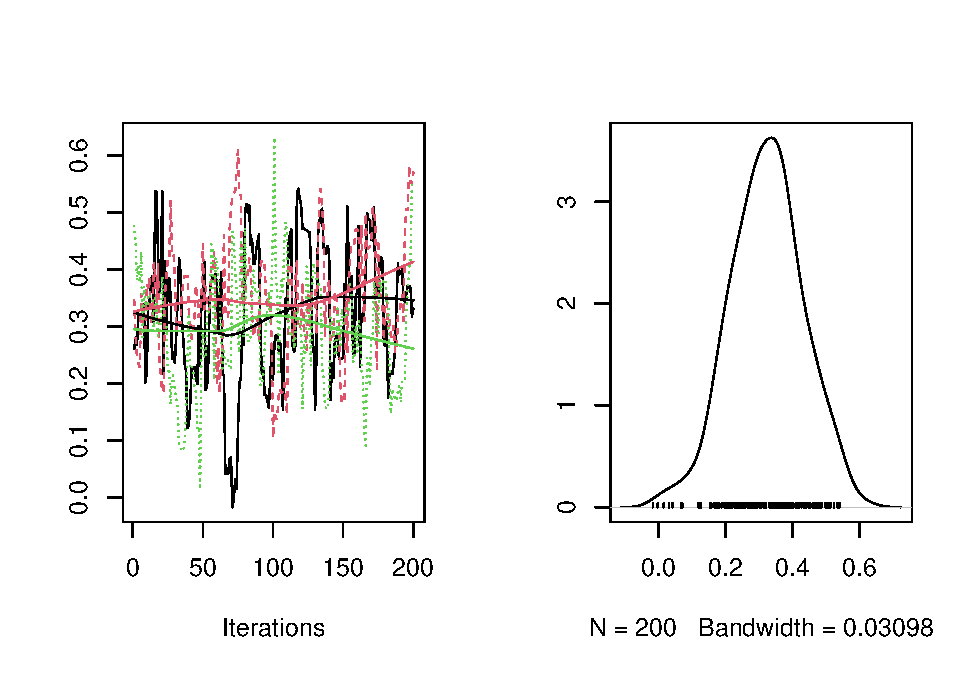
\includegraphics{Single_effect_files/figure-latex/function_HMC-1.pdf}

\begin{verbatim}
## Potential scale reduction factors:
## 
##      Point est. Upper C.I.
## [1,]       1.06        1.2
\end{verbatim}

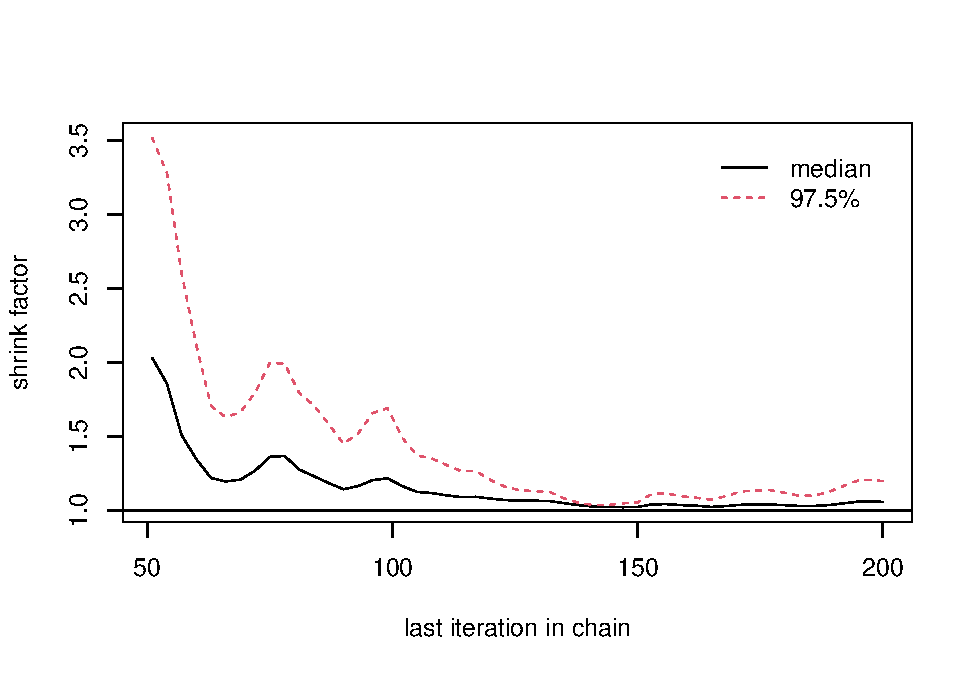
\includegraphics{Single_effect_files/figure-latex/function_HMC-2.pdf}
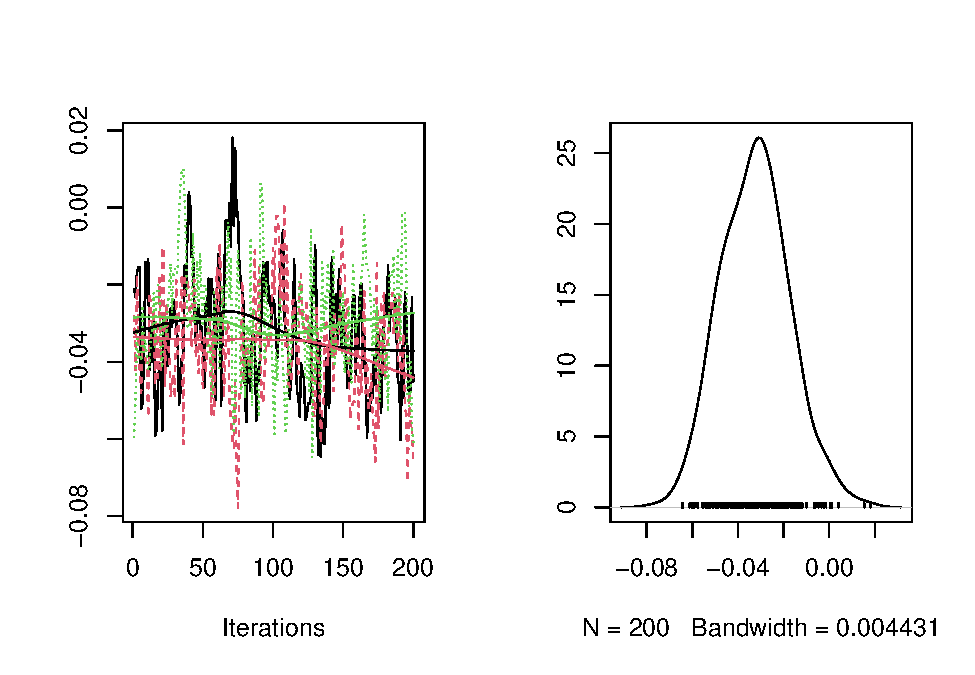
\includegraphics{Single_effect_files/figure-latex/function_HMC-3.pdf}

\begin{verbatim}
## Potential scale reduction factors:
## 
##      Point est. Upper C.I.
## [1,]       1.03       1.11
\end{verbatim}

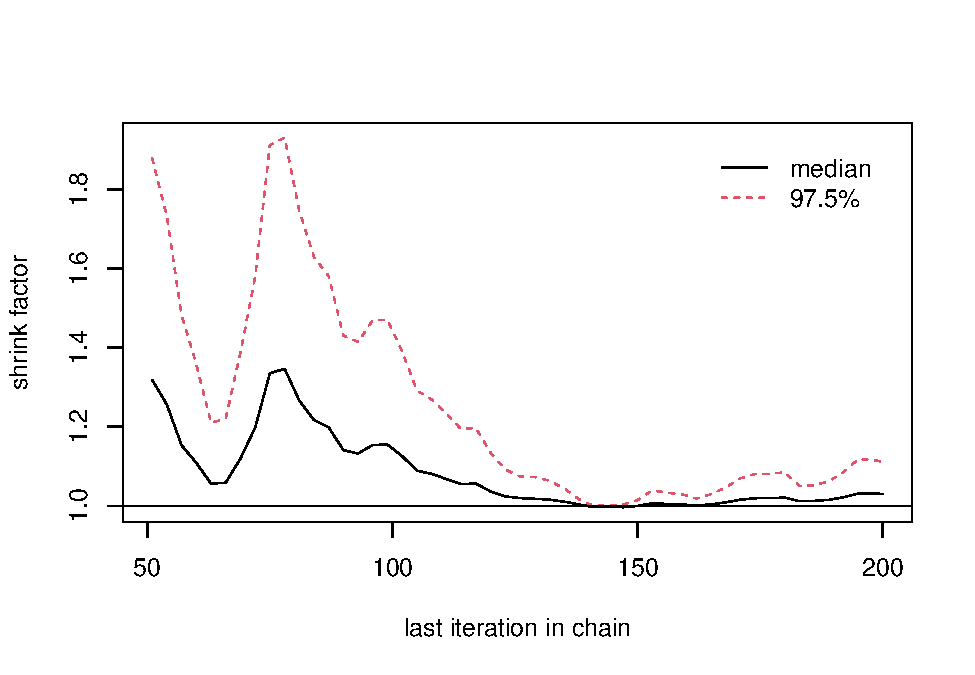
\includegraphics{Single_effect_files/figure-latex/function_HMC-4.pdf}

\begin{Shaded}
\begin{Highlighting}[]
\NormalTok{convergence}
\end{Highlighting}
\end{Shaded}

\begin{verbatim}
## $beta0_gelman
## [1] 1.056828
## 
## $beta1_gelman
## [1] 1.030134
\end{verbatim}

After the test for MCMC algorithm, we construct the BMA\_inference
algorithm based on NUTS and simple BMA. In addition, the function of
multiple chains to check convergence are also provided inside the whole
algorithm. If multiple chains are needed, then parallel computing for
sampling will be used.

\begin{Shaded}
\begin{Highlighting}[]
\CommentTok{# calculate log-likelihood for a pair of parameters.}
\NormalTok{log_logistic_likelihood =}\StringTok{ }\ControlFlowTok{function}\NormalTok{(x, y, beta_}\DecValTok{0}\NormalTok{, beta_}\DecValTok{1}\NormalTok{, }\DataTypeTok{tol =} \FloatTok{1e-100}\NormalTok{)\{}
\NormalTok{  lm =}\StringTok{ }\NormalTok{beta_}\DecValTok{0} \OperatorTok{+}\StringTok{ }\NormalTok{beta_}\DecValTok{1} \OperatorTok{*}\StringTok{ }\NormalTok{x}
  \KeywordTok{return}\NormalTok{(}\KeywordTok{sum}\NormalTok{(y }\OperatorTok{*}\StringTok{ }\KeywordTok{log}\NormalTok{(}\KeywordTok{sigmoid}\NormalTok{(lm) }\OperatorTok{+}\StringTok{ }\NormalTok{tol) }\OperatorTok{+}\StringTok{ }\NormalTok{(}\DecValTok{1} \OperatorTok{-}\StringTok{ }\NormalTok{y) }\OperatorTok{*}\StringTok{ }\KeywordTok{log}\NormalTok{(}\DecValTok{1} \OperatorTok{-}\StringTok{ }\KeywordTok{sigmoid}\NormalTok{(lm) }\OperatorTok{+}\StringTok{ }\NormalTok{tol)))}
\NormalTok{\}}



\CommentTok{# the main algorithm of Bayesian Model Averaging with Inference}
\CommentTok{# Input:}
\CommentTok{# X: a matrix of genotype data. The process of centralization or normalization should be calculated before this algorithm if needed.}
\CommentTok{# Y: a vector of phenotype data, only binary data(0 or 1) is allowed. }
\CommentTok{# prior_ip: prior inclusion probability for each model. The size of vector should be consistent with variables of X. If prior_ip is not normalized(sum to 1), a process of normalization will be done in algorithm.}
\CommentTok{# mu0: a scalar to specify the prior normal mean of beta_1}
\CommentTok{# sigma0: a scalar to specify the prior normal standard deviation of beta_1}
\CommentTok{# lower: a scalar to specify the prior lower bound of uniform distribution for beta_0}
\CommentTok{# higher: a scalar to specify the prior upper bound of uniform distribution for beta_0}
\CommentTok{# sample_size: a scalar to specify the number of samples for parameters to perform Monte Carlo Integral for p(data | M_j)}
\CommentTok{# n_chain : an integer to specify the number of chains needed in convergence diagnostics. And only the samples from the first chain will be returned.}
\CommentTok{# burn_n: an integer to specify the number of burn-in turns.}
\CommentTok{# sample_n: an integer to specify the number of samplers.}
\CommentTok{# sample_gap: an integer to specify the number of sampling gap, which mean we only get 1 samples from total gap samples. Basically, there are (sample_n * sample_gap) turns to sample after burn-in phrase.}
\CommentTok{# e: a scalar to specify the step size parameter in NUTS.}

\CommentTok{# output:}
\CommentTok{# A list. The first element is a vector of posterior inclusion probability for each variable. The second vector is Gelman-Rubin statistics and samples for each gene.}
\NormalTok{BMA_inference =}\StringTok{ }\ControlFlowTok{function}\NormalTok{(X, Y, prior_ip, mu0, sigma0, lower, higher, }\DataTypeTok{sample_size =} \DecValTok{10000}\NormalTok{, }\DataTypeTok{n_chain =} \DecValTok{3}\NormalTok{, }\DataTypeTok{burn_n =} \DecValTok{200}\NormalTok{, }\DataTypeTok{sample_n =} \DecValTok{200}\NormalTok{, }\DataTypeTok{sample_gap =} \DecValTok{1}\NormalTok{, }\DataTypeTok{e =} \FloatTok{0.01}\NormalTok{)\{}
\NormalTok{  n =}\StringTok{ }\KeywordTok{nrow}\NormalTok{(X)}
\NormalTok{  p =}\StringTok{ }\KeywordTok{ncol}\NormalTok{(X)}
  \ControlFlowTok{if}\NormalTok{(}\KeywordTok{length}\NormalTok{(prior_ip) }\OperatorTok{!=}\StringTok{ }\NormalTok{p)\{}
    \KeywordTok{stop}\NormalTok{(}\StringTok{"number of dimensions of prior inclusion probability and X are not consistent"}\NormalTok{)}
\NormalTok{  \}}
  \ControlFlowTok{if}\NormalTok{(}\KeywordTok{sum}\NormalTok{(prior_ip) }\OperatorTok{!=}\StringTok{ }\DecValTok{1}\NormalTok{)}
\NormalTok{    prior_ip =}\StringTok{ }\NormalTok{prior_ip }\OperatorTok{/}\StringTok{ }\KeywordTok{sum}\NormalTok{(prior_ip)}
\NormalTok{  beta_}\DecValTok{0}\NormalTok{ =}\StringTok{ }\KeywordTok{sapply}\NormalTok{(}\DecValTok{1}\OperatorTok{:}\NormalTok{p, }\ControlFlowTok{function}\NormalTok{(x)\{}\KeywordTok{runif}\NormalTok{(sample_size, lower, higher)\})}
\NormalTok{  beta_}\DecValTok{1}\NormalTok{ =}\StringTok{ }\KeywordTok{sapply}\NormalTok{(}\DecValTok{1}\OperatorTok{:}\NormalTok{p, }\ControlFlowTok{function}\NormalTok{(x)\{}\KeywordTok{rnorm}\NormalTok{(sample_size, mu0, sigma0)\})}
  
  
  
  \CommentTok{# parallel sampling}
  \KeywordTok{registerDoParallel}\NormalTok{(}\DecValTok{4}\NormalTok{)}
  
  \CommentTok{# run sampling algorithm for each gene}
\NormalTok{  chains =}\StringTok{ }\KeywordTok{sapply}\NormalTok{(}\DecValTok{1}\OperatorTok{:}\NormalTok{p, }\ControlFlowTok{function}\NormalTok{(j)\{}
    
    \CommentTok{# sample multiple chain}
\NormalTok{    multiple_chains =}\StringTok{ }\KeywordTok{foreach}\NormalTok{(}\DataTypeTok{i =} \DecValTok{1}\OperatorTok{:}\NormalTok{n_chain, }\DataTypeTok{.combine =}\NormalTok{ cbind) }\OperatorTok\StringTok{ }\NormalTok{\{}
\NormalTok{    beta0 =}\StringTok{ }\NormalTok{beta_}\DecValTok{0}\NormalTok{[i, j]}
\NormalTok{    beta1 =}\StringTok{ }\NormalTok{beta_}\DecValTok{1}\NormalTok{[i, j]}
    \KeywordTok{bayes_logit}\NormalTok{(burn_n, sample_n, sample_gap, x, Y, beta0, beta1, mu0, sigma0, lower, higher, e)}
\NormalTok{    \}}
    
\NormalTok{    result =}\StringTok{ }\KeywordTok{list}\NormalTok{()}
    \ControlFlowTok{if}\NormalTok{ (n_chain }\OperatorTok{==}\StringTok{ }\DecValTok{1}\NormalTok{) \{}
      \CommentTok{# if sample only one chain, then just return samples}
\NormalTok{      result[[}\StringTok{"beta_0_samples"}\NormalTok{]] =}\StringTok{ }\NormalTok{beta_}\DecValTok{0}\NormalTok{[[}\DecValTok{1}\NormalTok{]]}
\NormalTok{      result[[}\StringTok{"beta_1_samples"}\NormalTok{]] =}\StringTok{ }\NormalTok{beta_}\DecValTok{1}\NormalTok{[[}\DecValTok{1}\NormalTok{]]}
\NormalTok{      result[[}\StringTok{"beta_0_mean"}\NormalTok{]] =}\StringTok{ }\KeywordTok{mean}\NormalTok{(beta_}\DecValTok{0}\NormalTok{[[}\DecValTok{1}\NormalTok{]])}
\NormalTok{      result[[}\StringTok{"beta_1_mean"}\NormalTok{]] =}\StringTok{ }\KeywordTok{mean}\NormalTok{(beta_}\DecValTok{1}\NormalTok{[[}\DecValTok{1}\NormalTok{]])}
      \KeywordTok{return}\NormalTok{(result)}
\NormalTok{    \}}
    \ControlFlowTok{else}\NormalTok{\{}
      \CommentTok{# if sample for multiple chains, then Gelman-rubin`s statistics is calculated. The statistics and the samples from the first chain are returned.}
\NormalTok{      beta_}\DecValTok{0}\NormalTok{ =}\StringTok{ }\KeywordTok{list}\NormalTok{()}
\NormalTok{      beta_}\DecValTok{1}\NormalTok{ =}\StringTok{ }\KeywordTok{list}\NormalTok{()}
      \ControlFlowTok{for}\NormalTok{ (i }\ControlFlowTok{in} \DecValTok{1}\OperatorTok{:}\NormalTok{n_chain) \{}
\NormalTok{        beta_}\DecValTok{0}\NormalTok{[[i]] =}\StringTok{ }\NormalTok{multiple_chains[, i }\OperatorTok{*}\StringTok{ }\DecValTok{2} \OperatorTok{-}\StringTok{ }\DecValTok{1}\NormalTok{]}
\NormalTok{        beta_}\DecValTok{1}\NormalTok{[[i]] =}\StringTok{ }\NormalTok{multiple_chains[, i }\OperatorTok{*}\StringTok{ }\DecValTok{2}\NormalTok{]}
\NormalTok{      \}}
\NormalTok{      result =}\StringTok{ }\KeywordTok{HMC_convergence}\NormalTok{(beta_}\DecValTok{0}\NormalTok{, beta_}\DecValTok{1}\NormalTok{, }\DataTypeTok{plot_ =} \OtherTok{FALSE}\NormalTok{)}
\NormalTok{      result[[}\StringTok{"beta_0_samples"}\NormalTok{]] =}\StringTok{ }\NormalTok{beta_}\DecValTok{0}\NormalTok{[[}\DecValTok{1}\NormalTok{]]}
\NormalTok{      result[[}\StringTok{"beta_1_samples"}\NormalTok{]] =}\StringTok{ }\NormalTok{beta_}\DecValTok{1}\NormalTok{[[}\DecValTok{1}\NormalTok{]]}
\NormalTok{      result[[}\StringTok{"beta_0_mean"}\NormalTok{]] =}\StringTok{ }\KeywordTok{mean}\NormalTok{(beta_}\DecValTok{0}\NormalTok{[[}\DecValTok{1}\NormalTok{]])}
\NormalTok{      result[[}\StringTok{"beta_1_mean"}\NormalTok{]] =}\StringTok{ }\KeywordTok{mean}\NormalTok{(beta_}\DecValTok{1}\NormalTok{[[}\DecValTok{1}\NormalTok{]])}
      \KeywordTok{return}\NormalTok{(result)}
\NormalTok{    \}}
\NormalTok{  \})}
  
  
  \CommentTok{# calculate log-likelihood condition on only model}
\NormalTok{  logp_likelihood =}\StringTok{ }\KeywordTok{sapply}\NormalTok{(}\DecValTok{1}\OperatorTok{:}\NormalTok{p, }\ControlFlowTok{function}\NormalTok{(j)\{}
    \ControlFlowTok{if}\NormalTok{ (p }\OperatorTok{==}\StringTok{ }\DecValTok{1}\NormalTok{)\{}
\NormalTok{      beta_}\DecValTok{0}\NormalTok{_j =}\StringTok{ }\NormalTok{beta_}\DecValTok{0}
\NormalTok{      beta_}\DecValTok{1}\NormalTok{_j =}\StringTok{ }\NormalTok{beta_}\DecValTok{1}
\NormalTok{      x_j =}\StringTok{ }\NormalTok{X}
\NormalTok{    \}}\ControlFlowTok{else}\NormalTok{\{}
\NormalTok{      beta_}\DecValTok{0}\NormalTok{_j =}\StringTok{ }\NormalTok{beta_}\DecValTok{0}\NormalTok{[, j]}
\NormalTok{      beta_}\DecValTok{1}\NormalTok{_j =}\StringTok{ }\NormalTok{beta_}\DecValTok{1}\NormalTok{[, j]}
\NormalTok{      x_j =}\StringTok{ }\NormalTok{X[, j]}
\NormalTok{    \}}
\NormalTok{    log_likelihood_j =}\StringTok{ }\KeywordTok{log}\NormalTok{(}\KeywordTok{mean}\NormalTok{(}\KeywordTok{exp}\NormalTok{(}\KeywordTok{sapply}\NormalTok{(}\DecValTok{1}\OperatorTok{:}\NormalTok{sample_size, }\ControlFlowTok{function}\NormalTok{(i)\{}
      \KeywordTok{log_logistic_likelihood}\NormalTok{(x_j, Y, beta_}\DecValTok{0}\NormalTok{_j[i], beta_}\DecValTok{1}\NormalTok{_j[i])}
\NormalTok{    \}))))}
\NormalTok{    log_likelihood_j}
\NormalTok{  \})}
  
  \CommentTok{# calculate PIP}
\NormalTok{  logp_prior_ip =}\StringTok{ }\KeywordTok{log}\NormalTok{(prior_ip)}
\NormalTok{  posterior_ip =}\StringTok{ }\KeywordTok{softmax}\NormalTok{(logp_prior_ip }\OperatorTok{+}\StringTok{ }\NormalTok{logp_likelihood)}
  \KeywordTok{return}\NormalTok{(}\KeywordTok{list}\NormalTok{(posterior_ip, chains))}
\NormalTok{\}}

\CommentTok{# simulate}
\NormalTok{n =}\StringTok{ }\DecValTok{1000}
\NormalTok{X =}\StringTok{ }\KeywordTok{cbind}\NormalTok{(}\KeywordTok{rnorm}\NormalTok{(n, }\DecValTok{10}\NormalTok{), }\KeywordTok{rnorm}\NormalTok{(n, }\DecValTok{1}\NormalTok{), }\KeywordTok{rnorm}\NormalTok{(n, }\DecValTok{1}\NormalTok{, }\DecValTok{5}\NormalTok{))}
\NormalTok{X =}\StringTok{ }\NormalTok{X }\OperatorTok{-}\StringTok{ }\KeywordTok{colMeans}\NormalTok{(X)}
\NormalTok{b =}\StringTok{ }\KeywordTok{c}\NormalTok{(}\DecValTok{2}\NormalTok{,}\DecValTok{5}\NormalTok{,}\OperatorTok{-}\DecValTok{2}\NormalTok{)}
\NormalTok{Y =}\StringTok{ }\KeywordTok{rbinom}\NormalTok{(n, }\DecValTok{1}\NormalTok{, }\KeywordTok{sigmoid}\NormalTok{(X }\OperatorTok\StringTok{ }\NormalTok{b }\OperatorTok{+}\StringTok{ }\DecValTok{2}\NormalTok{))}
\NormalTok{result =}\StringTok{ }\KeywordTok{BMA_inference}\NormalTok{(X, Y, }\KeywordTok{rep}\NormalTok{(}\DecValTok{1}\OperatorTok{/}\KeywordTok{ncol}\NormalTok{(X), }\KeywordTok{ncol}\NormalTok{(X)), }\DecValTok{0}\NormalTok{, }\DecValTok{1}\NormalTok{, }\DecValTok{-10}\NormalTok{, }\DecValTok{10}\NormalTok{)}
\NormalTok{result}
\end{Highlighting}
\end{Shaded}

\begin{verbatim}
## [[1]]
## [1] 1.479029e-141  1.000000e+00  1.686970e-34
## 
## [[2]]
##                [,1]        [,2]        [,3]       
## beta0_gelman   1.013545    1.271711    1.031487   
## beta1_gelman   1.005131    1.206365    1.028493   
## beta_0_samples Numeric,200 Numeric,200 Numeric,200
## beta_1_samples Numeric,200 Numeric,200 Numeric,200
## beta_0_mean    0.2881341   0.3824781   0.2963373  
## beta_1_mean    -0.02890543 -0.04050875 -0.03051668
\end{verbatim}

\hypertarget{the-rest-of-notebook-has-not-been-completed-yet-and-will-be-done-a-few-days-later.}{%
\section{The rest of notebook has not been completed yet and will be
done a few days
later.}\label{the-rest-of-notebook-has-not-been-completed-yet-and-will-be-done-a-few-days-later.}}

\hypertarget{bayesian-variable-selection-based-logistic-regression}{%
\subsubsection{Bayesian Variable Selection based Logistic
Regression}\label{bayesian-variable-selection-based-logistic-regression}}

This a Hamilton Monte Carlo Implementation for ``Single effect''
Bayesian Logistic Regression. In some genetic background, we need to
find the association between a specific phenotype(disease or not) and a
set of genes. In traditional setting, logistic regression can be used to
cope with such problem. However, as the number of tested genes grows
very rapidly, traditional logistic regression has several backdrops,
that identifies very low association for each gene. In order to solve
this problem, Bayesian Variable Selection are applied to select the most
``significant'' genes. In some extreme situations, only one gene are
expected to be select.

In the fully-Bayesian model, vanilla logistic regression can be treated
as \(y \sim Bernoulli(sigmoid(b_0 + Xb))\), where
\(sigmoid(x) = \frac{1}{1 + exp(-x)}\). Introducing Variable Selection
technique, we add a new discrete variable \(g\), such that \(g_i\)
indicates the prior inclusion probability that \(b_i\) will be included
in regression model. Therefore, the whole likelihood will be
\(y \sim Bernoulli(sigmoid(b_0 + X(b \odot g)))\). Based on this model,
we set the prior of \(b_0\) as a flat prior which means
\(b_0 \varpropto 1\), and specify normal distribution for each \(b_j\)
as \(b_j \sim N(\mu_0, \sigma_0)\). Since \(g\) follows a discrete
variable, we specify a vector prior \(g_0\) for \(g\) where
\(\sum_ig_{0i} = 1\) and a discrete uniform distribution will be used as
default.

\hypertarget{simple-bayesian-logistic-regression}{%
\subsubsection{Simple Bayesian Logistic
Regression}\label{simple-bayesian-logistic-regression}}

To make the whole problem testable, we first implement a Hamilton Monte
Carlo(HMC) based vanilla logistic regression to fit the model. HMC is a
well-known Monte Carlo method based on Hmamilton Dynamic in Physics. An
brief introduction can be find
\href{https://en.wikipedia.org/wiki/Hamiltonian_Monte_Carlo}{here} . In
this algorithm, we need to calculate the derivative of log-posterior
distribution of each parameters.

\hypertarget{fully-bayesian-model}{%
\paragraph{Fully-Bayesian Model}\label{fully-bayesian-model}}

To get the complete fully-Bayesian model, we need to carefully write
down the likelihood function, prior and posterior distributions:

Likelihood:
\(f(Y|X,b_0, b) = \prod_i^n (sigmoid(b_0 + X_i(b \odot g)))^{y_i}(1 - sigmoid(b_0 + X_ib)))^{1 - y_i}\)

Prior: \(b_0 \varpropto 1\),
\(\pi(b_i) \varpropto exp(-\frac{(b_i - \mu_0)^2}{2\sigma_0^2})\)..

Fully Posterior:
\(p(Y, b_0, b | X) \varpropto \prod_i^n (sigmoid(b_0 + X_ib ))^{y_i}(1 - sigmoid(b_0 + X_ib))^{1 - y_i} * \prod_j^p exp(-\frac{(b_j - \mu_0)^2}{2\sigma_0^2})\)

Marginal Posterior:
\(p(b_0 | Y, b, X) \varpropto \prod_i^n (sigmoid(b_0 + X_ib ))^{y_i}(1 - sigmoid(b_0 + X_ib))^{1 - y_i}\),
\$p(b\_j \textbar{} Y, b\_0, X) \varpropto \prod\_i\^{}n (sigmoid(b\_0 +
X\_ib ))\^{}\{y\_i\}(1 - sigmoid(b\_0 + X\_ib))\^{}\{1 - y\_i\} *
exp(-\frac{(b_j - \mu_0)^2}{2\sigma_0^2}) \$

\hypertarget{fully-bayesian-model-1}{%
\subsubsection{Fully-Bayesian Model}\label{fully-bayesian-model-1}}

To get the complete fully-Bayesian model, we need to carefully write
down the likelihood function, prior and posterior distributions:

Likelihood:
\(f(Y|X,b_0, b, g) = \prod_i^n (sigmoid(b_0 + X_i(b \odot g)))^{y_i}(1 - sigmoid(b_0 + X_i(b \odot g)))^{1 - y_i}\)

Prior: \(b_0 \varpropto 1\),
\(\pi(b_i) = \frac{1}{\sqrt{2\pi}\sigma_0}exp(-\frac{(b_i - \mu_0)^2}{2\sigma_0^2})\),
\(\pi(g_{0i}) = \frac{1}{p}\), where \(p\) stands for the number of
predictors.

Fully Posterior:
\(p(Y, b_0, b, g | X) \varpropto \prod_i^n (sigmoid(b_0 + X_i(b \odot g)))^{y_i}(1 - sigmoid(b_0 + X_i(b \odot g)))^{1 - y_i} * \prod_i^p \frac{1}{\sigma_0}exp(-\frac{(b_i - \mu_0)^2}{2\sigma_0^2})\)

Marginal Posterior: \(p(b_0)\)

\end{document}
